% !TeX program = xelatex
\documentclass[UTF8,fontset=fandol,11pt,a4paper]{ctexart}
\usepackage[margin=2.4cm,headheight=15pt]{geometry}
\usepackage{amsmath,amssymb,bm,mathtools,newtxtext,newtxmath}
\usepackage{graphicx,booktabs,tabularx,array,placeins,microtype,fancyhdr}
\usepackage[font=small,labelfont=bf,labelsep=quad]{caption}
\usepackage{xurl}
\usepackage[colorlinks=true,linkcolor=black,citecolor=black,urlcolor=black]{hyperref}
\linespread{1.15}\setlength{\parskip}{.15em}\setlength{\emergencystretch}{2em}
\graphicspath{{figures/}}\pagestyle{fancy}\fancyhf{}
\fancyhead[L]{\small 变质量火箭的轨道规划与预测控制}
\fancyhead[R]{\small 启发式优化对比研究}\fancyfoot[C]{\thepage}
\newcommand{\dd}{\,\mathrm d}
\newcommand{\bvec}[1]{\bm{#1}}
\newcommand{\unit}[1]{\,\mathrm{#1}}
\newcommand{\PSOPass}{5}
\newcommand{\PSOMedian}{\ensuremath{1.75\times10^{-6}}}
\newcommand{\GAPass}{0}
\newcommand{\GAMedian}{\ensuremath{2.29\times10^{-4}}}
\newcommand{\SAPass}{0}
\newcommand{\SAMedian}{\ensuremath{5.22\times10^{-3}}}
\newcommand{\ClosedPos}{1.945}
\newcommand{\OpenPos}{25836.6}
\newcommand{\ClosedVel}{0.0976}
\newcommand{\OpenVel}{106.668}
\newcommand{\MaxFineRadius}{0.199}
\newcommand{\ReferenceSeed}{161}
\newcommand{\ReferenceTime}{522.284}
\newcommand{\ReferenceFuel}{53547.1}
\newcommand{\ReferenceHeight}{-8.125}
\newcommand{\ReferenceRadial}{-0.0486}
\newcommand{\ReferenceTangential}{0.0288}
\newcommand{\QPCount}{259}
\newcommand{\QPFail}{0}
\newcommand{\QPMean}{4.555}
\newcommand{\QPMax}{589.9}

\title{\heiti 变质量火箭两段燃烧轨道规划的启发式优化比较\\与模型预测控制}
\author{金承果}\date{}
\begin{document}\maketitle
\begin{abstract}
针对变推力、变质量火箭的近地圆轨道注入问题，建立含中心引力、二次空气阻力和密度相关高斯扰动的二维极坐标动力学模型，构建离线规划与在线轨迹跟踪的分层框架。以两段燃烧及中间滑行为控制结构，将偏角、流率和阶段时长参数化为十维变量。在相同初始候选、搜索边界、扰动实现及评价预算下，对纯粒子群优化（PSO）、实数编码遗传算法（GA）和多起点模拟退火（SA）开展五组配对种子实验，全部算法均不使用局部精修。搜索采用并行四阶龙格--库塔积分，最终控制由独立高精度自适应积分复核。
在600\,km算例中，PSO、GA和SA的复核通过数分别为\PSOPass、\GAPass 和\SAPass（各五次），复核目标中位数分别为\PSOMedian、\GAMedian 和\SAMedian。以通过复核的纯PSO轨迹为参考，构造时变线性化MPC并求解凸二次规划。在独立于规划的同一实际扰动下，闭环与开环位置跟踪均方根误差分别为\ClosedPos\,m和\OpenPos\,m。
结果支持在本模型、预算及配置下比较三种搜索策略，并表明滚动反馈能抑制参考执行中的误差积累。有限重复试验不构成算法一般优越性或严格闭环稳定性的证明。
\vspace{.4em}\par\noindent\textbf{关键词：}变质量动力学；两段燃烧；粒子群优化；遗传算法；模拟退火；模型预测控制；二次规划
\end{abstract}
\section{引言}
近地轨道是对地观测、空间实验和航天运输的重要运行区域。入轨不仅要求给定高度，还要求位置与速度同时满足轨道条件。齐奥尔科夫斯基方程描述理想推进能力与质量比的关系\cite{tsiolkovsky1903,sutton2016}，但不能直接给出包含引力、阻力和有限推力转向的实际轨迹。

控制参数化与动力学积分可将入轨问题转化为有限维非线性优化。PSO通过个体与群体经验搜索\cite{kennedy1995pso}，GA通过选择与重组传播候选信息\cite{holland1992}，SA利用温度相关概率接受规则探索非凸目标\cite{kirkpatrick1983}。表现依赖边界、初始点及计算预算，单次最好结果不足以支持方法间比较；附加局部精修还会混合不同算法的贡献。

离线可行轨迹也不保证在新扰动下准确开环执行。MPC通过反馈、有限时域预测和约束优化修正输入\cite{mayne2000mpc,borrelli2017}，适合协调参考附近的状态误差与控制边界。

本文在统一动力学和两段燃烧参数化下比较无局部精修的PSO、GA和SA，区分搜索评价与高精度复核。随后以纯PSO轨迹构造时变线性化MPC，检验同一实际扰动下的开闭环差异。结论限于单级质点算例及所用实现，不作算法一般性排序或工程适用性声明。

\section{变质量火箭的动力学模型}
\subsection{理想推进关系与质量比下界}
设质量为$m$，相对排气速度大小为$c$，排出质量为$-\mathrm dm>0$。微元动量平衡为
\begin{equation}m\mathrm dv=-c\mathrm dm+F_{\rm ext}\mathrm dt.\end{equation}
忽略外力且$c$恒定时，
\begin{equation}\Delta v_{\rm ideal}=c\ln(m_0/m_f),\qquad I_T=\int_0^{t_f}T\dd t=c(m_0-m_f).\label{eq:tsiolkovsky}\end{equation}
速度增量涉及$\int T/m\dd t$，不能以总冲量除以初始质量代替。

目标半径$r_*=R_E+h_*$、圆轨道速度$v_c=\sqrt{\mu/r_*}$。对从$r_0$静止出发且$r\ge r_0$的确定性轨迹，令
\begin{equation}\mathcal E=V^2/2+\mu(1/r_0-1/r).\end{equation}
无随机外力且阻力耗能时，$\dot{\mathcal E}\le(T/m)V\le(T/m)\sqrt{2\mathcal E}$。积分并代入圆轨道末态得到
\begin{equation}\frac{m_0}{m_f}\ge\exp\left[\frac1c\sqrt{\frac{2\mu}{r_0}-\frac{\mu}{r_*}}\right].\end{equation}
算例中该界约为6.245，仅用于能力筛查；它不是充分可行条件，也不对任意高斯外力样本成立。

\subsection{二维极坐标运动方程}
地球取不旋转球对称引力源，火箭取固定惯性平面内的变质量质点。忽略升力、分级与姿态执行机构动态。定义
\begin{equation}h=r-R_E,\quad u=\dot r,\quad w=r\dot\theta,\quad V=\sqrt{u^2+w^2},\quad\beta=\operatorname{atan2}(w,u).\end{equation}
控制为推力相对速度方向的偏角$\delta$及流率$q=-\dot m\ge0$，故$T=cq$、$\alpha=\beta+\delta$。起飞前5\,s保持$\alpha=0$，零速度附近采用方向保护。状态$x=(r,\theta,u,w,m,I_T)^{\mathsf T}$满足
\begin{equation}
\begin{aligned}
\dot r&=u,&\dot\theta&=w/r,\\
\dot u&=\frac{w^2}{r}+\frac{cq\cos\alpha}{m}-\frac{\mu}{r^2}-\frac{kVu}{m}+a_{\varepsilon,r},\\
\dot w&=-\frac{uw}{r}+\frac{cq\sin\alpha}{m}-\frac{kVw}{m}+a_{\varepsilon,\theta},\\
\dot m&=-q,&\dot I_T&=cq .
\end{aligned}\label{eq:dynamics}
\end{equation}
其中$\rho(h)=\rho_0e^{-\max(h,0)/H_a}$、$k=\rho C_DA_f/2$。阻力矢量为$-kV(u\bm e_r+w\bm e_\theta)$，大小为$kV^2$，在静止大气假设下与惯性速度反向。$w^2/r$与$-uw/r$为坐标运动学项，不是附加外力。优化允许主动偏角，不将全程视为严格零偏角重力转弯。

\subsection{密度相关随机激励}
\begin{equation}a_{\varepsilon,j}(t,h)=\sigma_{0,j}\frac{\rho(h)}{\rho_{\rm ref}}\eta_j(t),\quad j\in\{r,\theta\}.\label{eq:noise}\end{equation}
在间隔1\,s的网格上生成独立标准高斯样本$\xi_{j,\ell}$，作方差归一化插值：
\begin{equation}\eta_j(t)=\frac{(1-\lambda)\xi_{j,\ell}+\lambda\xi_{j,\ell+1}}{\sqrt{(1-\lambda)^2+\lambda^2}},\quad\lambda=t-\lfloor t\rfloor.\end{equation}
该过程具有有限时间相关性和单位边缘方差，可作为固定样本路径上的ODE激励。它不是理想白噪声；归一化因子使插值后过程也不是严格分段线性。扰动标准差与密度成正比，方差与密度平方成正比。

\section{数值积分与独立复核}
给定控制后，式\eqref{eq:dynamics}构成非线性初值问题。搜索阶段使用双精度RK4、最大步长0.05\,s；取整步数后均匀调整步长，使末点与计划关机时刻一致。启停使用0.5\,s线性过渡。三算法共用积分器和同一预生成扰动样本。

最终控制保持不变，使用Dormand--Prince自适应积分\cite{dormand1980,shampine1997}作两档复核：最大步长与相对容差分别为$(0.2\,\mathrm s,10^{-10})$和$(0.1\,\mathrm s,10^{-11})$。分量绝对容差随数据保存。细化差值检查数值敏感性，不视为严格误差上界。

预算在积分前检查；自适应积分检测燃尽与落地，燃尽后切换至无推力运动，落地则终止。验收要求高度误差不超过500\,m、径向及切向速度误差各不超过10\,m/s，同时满足燃料预算且未触地。验收容差不等于搜索目标归一化尺度。

正式搜索共用16线程编译积分内核，MATLAB负责最终复核及MPC。另实现RTX 5060双精度CUDA核，与多核实现对同一96个候选的最大终态分量差约为$1.9\times10^{-9}$、目标最大差约为$8.4\times10^{-12}$。本机此小批量试算中多核实现更快，故正式比较统一用多核后端。计时排除编译与预热，不外推为其他硬件或批量下的性能排序。

\section{两段燃烧规划与对比算法}
\subsection{控制参数化与优化目标}
采用两段燃烧及中间滑行结构，将连续控制函数压缩为十维设计向量：
\begin{equation}z=(\delta_1,\delta_2,\delta_3,\delta_4,\delta_5,q_1,q_2,t_1,t_c,t_2)^{\mathsf T}.\end{equation}
其中，前五项描述偏角节点，其余变量给出两段平台流率及燃烧、滑行时长。第一段偏角节点位于$0.2t_1$、$0.6t_1$和关机过渡起点，第二段偏角由$\delta_4$逐步过渡至$\delta_5$。节点之间采用线性插值，滑行段流率严格为零，启停过程保留有限时长过渡。

在$\xi\in[0,1]^{10}$搜索，$z=z_{\rm lb}+\xi\odot(z_{\rm ub}-z_{\rm lb})$。边界为
\begin{equation}
\begin{aligned}
z_{\rm lb}&=(0,-15,-15,-15,-15,180,120,80,20,25),\\
z_{\rm ub}&=(15,15,15,15,15,350,350,240,400,150).
\end{aligned}
\end{equation}
角度、流率和时间单位分别为度、kg/s和s。规划要求终端状态接近目标圆轨道，不限定注入位置的极角，采用以下归一化误差目标：
\begin{equation}
J(z)=\left(\frac{h_f-h_*}{10^4\,{\rm m}}\right)^2+
\left(\frac{u_f}{10^3\,{\rm m/s}}\right)^2+
\left(\frac{w_f-v_c}{10^3\,{\rm m/s}}\right)^2.\label{eq:J}
\end{equation}
燃料超限返回$10^3+[(M_{\rm used}-M_{\rm budget})/(10^3\,{\rm kg})]^2$；触地则加$100+(t_f-t_{\rm impact})/(1\,{\rm s})$。目标不含燃料、时间、动压或过载最小项，因此不同解的资源差异不代表算法直接优化了这些指标。

\subsection{粒子群优化}
PSO按个体最佳$p_i$和群体最佳$g$更新\cite{kennedy1995pso}：
\begin{equation}
\begin{aligned}
\nu_i^{k+1}&=\omega_k\nu_i^k+c_1r_1\odot(p_i-\xi_i^k)+c_2r_2\odot(g-\xi_i^k),\\
\xi_i^{k+1}&=\mathcal R(\xi_i^k+\nu_i^{k+1}).
\end{aligned}
\end{equation}
$\mathcal R$反射修复边界。采用全局最佳拓扑，$\omega_k$由1.1线性降至0.1，$c_1=c_2=1.49$，速度限制$[-0.2,0.2]$。上述设置在统一评价预算下执行，以比较群体搜索对终端误差的降低能力。

\subsection{实数编码遗传算法}
GA采用实数染色体、三元锦标赛、混合算术交叉和高斯变异\cite{holland1992}。父代$a,b$生成
\begin{equation}\xi'=\gamma\odot a+(1-\gamma)\odot b,\quad\gamma_\ell\sim U(-0.25,1.25).\end{equation}
交叉后，各坐标以$1/10$的概率增加标准差为0.1的高斯扰动，并通过反射处理越界。每代保留一个历史最优个体，以维持已获得的搜索精度；该精英的重新评价计入总预算。

\subsection{多起点模拟退火}
SA设置96条独立链，每轮各链扰动一个随机坐标，按Metropolis规则接受\cite{kirkpatrick1983}：
\begin{equation}P_{\rm accept}=\min\{1,\exp[-(J(\xi')-J(\xi))/T_k]\}.\end{equation}
温度由1按几何序列降至$10^{-6}$，提议标准差由0.2线性降至0.005。各链独立更新、不交换状态，最终返回全部访问点中的历史最优解。该设置将相同初始候选用于多起点搜索，与单链退火及并行回火分别对应不同的实验协议。

\subsection{等预算配对设计}
每方法使用96个候选（SA为96条链）、180轮更新，总评价$96(180+1)=17376$次。种子161--165形成五组配对实验；组内初始点逐元素一致，一半均匀随机，一半按两段燃烧燃料分配启发式生成。后续算法使用独立可复现随机流，规划扰动固定为20261020。

各次运行均在固定预算耗尽后终止，并将搜索历史最优点提交至两档高精度复核。复核仅评价固定控制，不引入局部最小化或参数再搜索。性能指标包括完整收敛曲线、终端残差、目标中位数、四分位范围及验收通过数。配对种子用于观察优化器随机性，而实际扰动环境保持一致。

\section{时变线性化模型预测控制}
\subsection{参考与离散误差模型}
从通过验收的纯PSO结果中选择复核目标最小者作为参考，不施加任何局部精修。参考包含$\bar x(t)=(r,\theta,u,w,m)^{\mathsf T}$和$\bar\delta(t),\bar q(t)$；预测窗口超出计划关机时刻后，参考继续按无推力、无随机外力的动力学延伸。

采样周期$T_s=2$\,s、预测步数$N=15$。本周期施加$\delta(t)=\bar\delta(t)+\Delta\delta_k$、$q(t)=\bar q(t)+\Delta q_k$，其中修正$c_k=(\Delta\delta_k,\Delta q_k)^{\mathsf T}$保持常数，参考前馈仍连续变化。以RK4积分名义方程得到离散映射$F_k(x,c)$，沿参考展开并归一化：
\begin{equation}e_{k+1}=A_ke_k+B_kv_k+d_k,\label{eq:ltv}\end{equation}
\begin{equation}
\begin{aligned}
e_k&=S_x^{-1}(x_k-\bar x_k),&v_k&=S_c^{-1}c_k,\\
A_k&=S_x^{-1}F_{x,k}S_x,&B_k&=S_x^{-1}F_{c,k}S_c,\\
d_k&=S_x^{-1}[F_k(\bar x_k,0)-\bar x_{k+1}].
\end{aligned}
\end{equation}
$F_{x,k},F_{c,k}$由离散映射中心差分获得。状态尺度为$(500\,\mathrm m,500\,\mathrm m/R_E,30\,\mathrm{m/s},30\,\mathrm{m/s},1000\,\mathrm{kg})$，输入尺度为$(2^\circ,50\,\mathrm{kg/s})$。$d_k$保留参考插值、积分和名义扰动环境差异，不能解释为未来实际噪声预测。名义预测不读取实际未来扰动。

\subsection{代价凝聚与凸二次规划}
未来状态及控制堆叠为$E,U$，则式\eqref{eq:ltv}递推得到
\begin{equation}E=\mathcal A e_k+\mathcal B U+\mathcal D=a+\mathcal B U.\end{equation}
取有限时域目标
\begin{equation}
\begin{aligned}
J_{\rm MPC}={}&E^{\mathsf T}\bar Q E+U^{\mathsf T}\bar R U\\
&+(DU-b_\Delta)^{\mathsf T}\bar R_\Delta(DU-b_\Delta)
+\lambda_\epsilon\epsilon^{\mathsf T}\epsilon .
\end{aligned}
\end{equation}
$D$为控制差分矩阵，$b_\Delta$第一块为上步已执行修正。状态权重$Q=\operatorname{diag}(4,2,4,4,0.1)$，末步权重为$5Q$，$R=0.2I_2$，$R_\Delta=0.5I_2$，$\lambda_\epsilon=10^5$。惩罚的是反馈修正变化，不是总控制的硬性变化率限制。

令$\zeta=(U^{\mathsf T},\epsilon^{\mathsf T})^{\mathsf T}$，消去状态并去除常数项，得到
\begin{equation}\min_\zeta\tfrac12\zeta^{\mathsf T}H\zeta+f^{\mathsf T}\zeta,\quad G\zeta\le b,\quad l\le\zeta\le u,\end{equation}
其中
\begin{equation}
\begin{aligned}
H&=\operatorname{blkdiag}\left(2[\mathcal B^{\mathsf T}\bar Q\mathcal B+\bar R+D^{\mathsf T}\bar R_\Delta D],2\lambda_\epsilon I_N\right),\\
f&=\begin{bmatrix}2(\mathcal B^{\mathsf T}\bar Q a-D^{\mathsf T}\bar R_\Delta b_\Delta)\\0\end{bmatrix}.
\end{aligned}
\end{equation}
因$\bar R\succ0$、$\bar Q,\bar R_\Delta\succeq0$，目标严格凸\cite{boyd2004}。状态选择矩阵$C_r,C_m$分别提取径向及质量误差；参考高度和燃料余量归一化为$g,b_m$后，
\begin{equation}
G=\begin{bmatrix}-C_r\mathcal B&-I_N\\-C_m\mathcal B&0\end{bmatrix},\quad
b=\begin{bmatrix}g+C_ra\\b_m+C_ma\end{bmatrix},\quad\epsilon\ge0.
\end{equation}
地面为软约束，干质量为硬约束；输入限制$|\delta|\le15^\circ$、$0\le q\le350$\,kg/s，修正幅度限制$|\Delta\delta|\le5^\circ$、$|\Delta q|\le100$\,kg/s。滑行及关机后不新增点火。当前QP含$2N+N=45$个变量，以凸内点法求解。

每次仅执行第一项修正，下一周期更新状态后重算。起飞后首次反馈在6\,s施加。假设理想全状态测量，不包含传感器或执行机构动态；QP失败时退回参考前馈。该回退不构成一般安全性保证，局部QP凸性也不意味着原非线性控制问题具有全局最优性或递归可行性。

\section{结果与分析}
\subsection{实验设置与评价指标}
目标高度600\,km，初始质量60000\,kg、干质量1200\,kg、有效排气速度4500\,m/s。地球半径6371\,km、引力参数$3.986004418\times10^{14}$\,m$^3$/s$^2$；$\rho_0=\rho_{\rm ref}=1.225$\,kg/m$^3$、$H_a=8500$\,m、$C_D=0.35$、$A_f=2$\,m$^2$，两向参考扰动标准差均为0.1\,m/s$^2$。实验依次评价三种规划器的收敛与终端求解性能、搜索结果的数值敏感性，以及纯PSO参考在新扰动下的开闭环执行精度。

\subsection{无精修规划器对比}
本组实验比较三种算法在相同计算预算下获得可行入轨轨迹的能力。每种算法执行五次配对运行，每次使用17376次搜索评价，最终两次独立ODE复核作为统一的额外验收开销。表\ref{tab:algorithm}汇总高精度复核统计，图\ref{fig:algorithm}给出随评价次数变化的搜索目标中位数、四分位区间及全部最终复核值。
\begin{table}[htbp]\centering\small
\caption{等预算无精修比较（每种算法五次）。IQR为25\%--75\%区间，耗时不含编译与复核。}\label{tab:algorithm}
\begin{tabular}{lcccc}\toprule
算法 & 复核目标中位数 & IQR & 通过数 & 耗时中位数/s\\\midrule
PSO & \ensuremath{1.75\times10^{-6}} & [\ensuremath{1.22\times10^{-6}}, \ensuremath{2.32\times10^{-6}}] & 5/5 & 3.24\\
GA & \ensuremath{2.29\times10^{-4}} & [\ensuremath{1.90\times10^{-4}}, \ensuremath{5.49\times10^{-4}}] & 0/5 & 3.24\\
SA & \ensuremath{5.22\times10^{-3}} & [\ensuremath{2.70\times10^{-4}}, \ensuremath{9.26\times10^{-3}}] & 0/5 & 2.46\\
\bottomrule\end{tabular}\end{table}
\begin{figure}[htbp]\centering
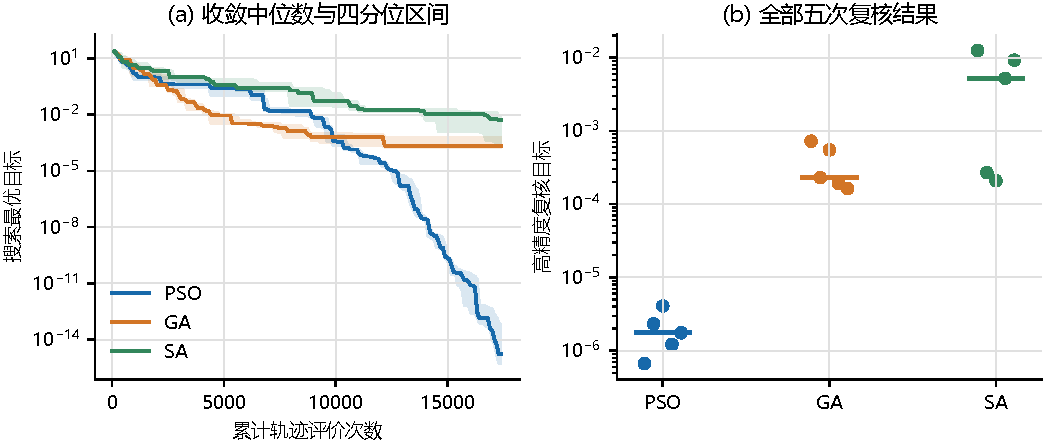
\includegraphics[width=.95\linewidth]{fig_planner_comparison.pdf}
\caption{等预算搜索与复核。左：搜索目标中位数及25\%--75\%区间；右：五个配对种子的高精度复核目标。搜索曲线与右图使用不同精度评价，不应直接等同。}\label{fig:algorithm}
\end{figure}
在当前预算与配置下，PSO的五次运行均通过高精度验收，而GA与SA的通过数均为0/5。表\ref{tab:algorithm}中，PSO的复核目标中位数低于GA和SA，说明其在本组实验中获得了更小的终端综合误差。图\ref{fig:residual}进一步显示，GA与SA虽然降低了目标值，但部分速度残差仍超过10\,m/s，成为未通过验收的主要原因。这表明归一化平方和与逐分量可行性应结合评价；单一目标值不能替代终端条件检查。
\begin{figure}[htbp]\centering
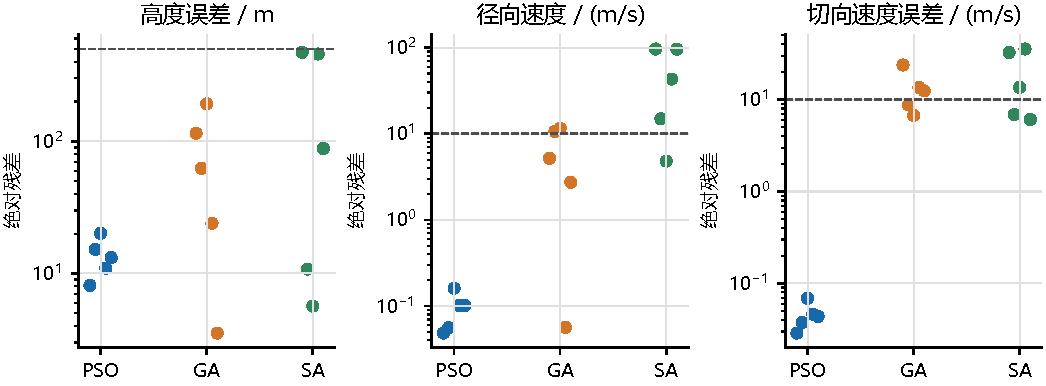
\includegraphics[width=.95\linewidth]{fig_planner_residuals.pdf}
\caption{最终候选的高精度复核残差。每点对应一次运行；虚线为高度500\,m和两速度10\,m/s验收界限。}\label{fig:residual}
\end{figure}

\subsection{搜索精度与参考轨迹}
搜索曲线与高精度复核结果之间存在明显的量级差异。PSO在定步长模型上的目标可降至极小值，而复核后的高度残差仍处于数米至数十米范围。这一差异说明，即使搜索器在离散模型上获得极小目标值，也不意味着连续动力学的终端误差同步趋近于零。因此，本文以高精度复核值作为入轨性能依据。进一步细化自适应积分后，终端径向差的最大值为\MaxFineRadius\,m，用于表征最终结果的数值敏感性。

选作MPC参考的PSO种子为\ReferenceSeed，关机时刻\ReferenceTime\,s，推进剂消耗\ReferenceFuel\,kg，高度、径向及切向速度残差分别为\ReferenceHeight\,m、\ReferenceRadial\,m/s和\ReferenceTangential\,m/s。其两段燃烧、滑行及状态演化见图\ref{fig:reference}。
\begin{figure}[htbp]\centering
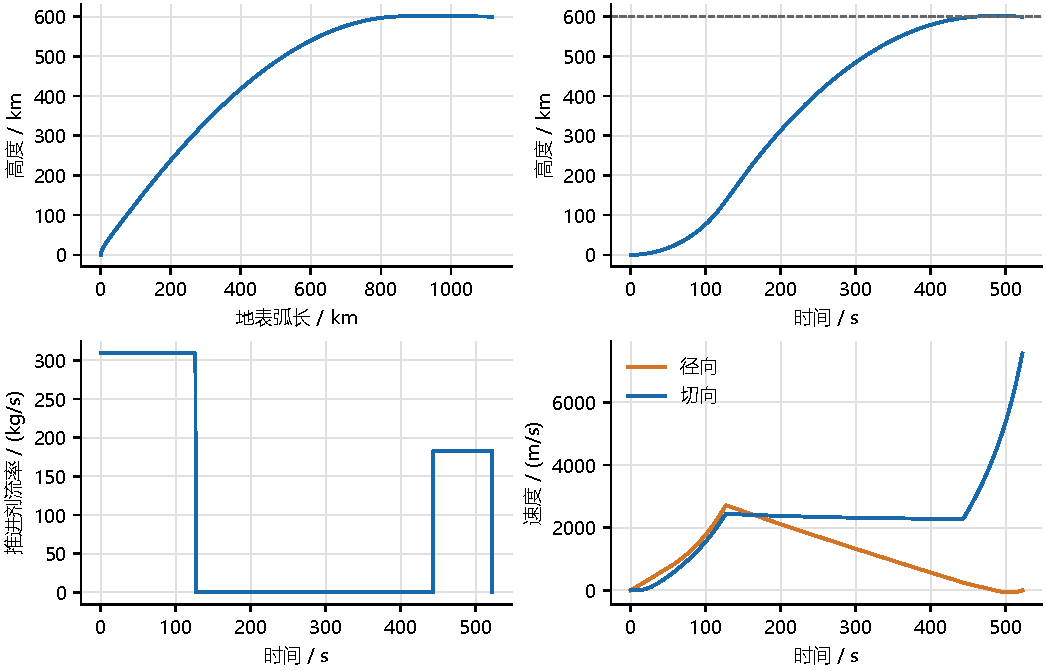
\includegraphics[width=.88\linewidth]{fig_pure_reference.pdf}
\caption{无局部精修的PSO参考：平面轨迹、高度、流率与速度时间历程。高度到达目标与速度完成圆轨化为不同要求。}\label{fig:reference}
\end{figure}
图\ref{fig:reference}展示了两段燃烧方案的阶段特征：第一段建立上升运动并积累横向速度，滑行段继续抬升高度，第二段则调节径向与切向速度以接近圆轨道条件。参考控制直接取自PSO返回参数，复核仅重新计算其动力学响应。

\subsection{独立扰动下的开闭环对照}
本组实验检验MPC对参考轨迹执行偏差的补偿作用。规划扰动种子为20261020，实际飞行采用20261021，以区分规划环境与验证环境。开环与闭环保持相同初值及实际扰动，前者执行参考前馈，后者叠加MPC反馈修正。在控制采样点上定义
\begin{equation}
E_p=\sqrt{\frac1M\sum_{j=1}^M[(r_j-\bar r_j)^2+R_E^2(\theta_j-\bar\theta_j)^2]},\quad
E_v=\sqrt{\frac1M\sum_{j=1}^M[(u_j-\bar u_j)^2+(w_j-\bar w_j)^2]} .
\end{equation}
其中，$E_p$合成径向误差与地表弧长误差，用于衡量沿参考轨迹的空间偏差。表\ref{tab:mpc}分别报告相对参考的跟踪RMS和相对目标圆轨道的关机误差，以区分轨迹执行精度与轨道注入精度。
\begin{table}[H]\centering\small
\caption{纯PSO参考的开闭环对照。}\label{tab:mpc}
\begin{tabular}{lrr}\toprule
指标 & 开环 & MPC\\\midrule
位置跟踪RMS / m & 25836.5824 & 1.9446\\
速度跟踪RMS / (m/s) & 106.6680 & 0.0976\\
关机高度误差 / m & -29848.9667 & -8.1569\\
关机径向速度 / (m/s) & -174.7328 & 0.0036\\
关机切向速度误差 / (m/s) & 101.7313 & 0.7456\\
\bottomrule\end{tabular}\end{table}
\begin{figure}[htbp]\centering
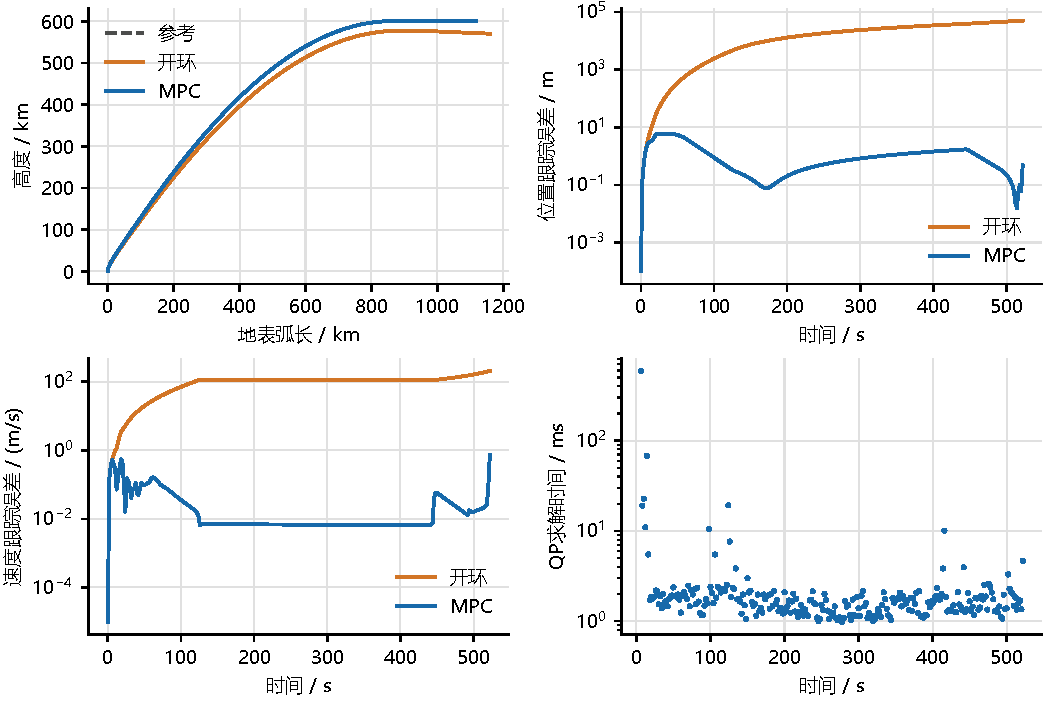
\includegraphics[width=.90\linewidth]{fig_pure_mpc.pdf}
\caption{相同实际扰动下的开环与MPC：平面轨迹、位置跟踪误差、速度跟踪误差及QP求解时间。对数误差图的零值显示下限仅用于绘图。}\label{fig:mpc}
\end{figure}
由表\ref{tab:mpc}与图\ref{fig:mpc}可见，MPC将位置跟踪RMS从开环的\OpenPos\,m降至\ClosedPos\,m，速度跟踪RMS从\OpenVel\,m/s降至\ClosedVel\,m/s。开环偏差随飞行过程积累，闭环则通过持续更新偏角与流率修正使轨迹保持在参考附近。该对照说明，性能改善来自状态反馈对执行偏差的补偿，而非初始状态或实际扰动条件的改变。参考轨迹自身仍具有非零入轨残差，因此较小的跟踪误差不意味着相对于目标轨道的误差同样为零。

在线过程中共求解\QPCount 次QP，失败\QPFail 次。单次平均耗时为\QPMean\,ms，最大耗时为\QPMax\,ms，均不包含参考线性化预计算。该结果表明，所构造的低维QP能够在本机桌面环境下完成滚动控制计算；嵌入式实现仍需结合目标硬件、测量开销和最坏情况时延进行独立评估。

\section{讨论}
\subsection{比较的有效范围}
对比控制了初始候选、边界、动力学、扰动样本与评价预算，移除了局部精修对终端误差的混合影响。PSO在当前参数下更充分地利用群体搜索信息；GA的变异和SA的提议温度、步长并未针对该目标调优。因此结果应表述为实现和配置的比较，而非优化范式的优劣证明。多起点SA返回96条链中的最好访问点，不能与同预算之外的单链结果直接混用。

五组配对种子的样本量有限，本文报告全部点、中位数及四分位范围，不将通过数解释为真实飞行成功概率，也不据此作总体显著性声明。全部规划共用一个扰动实现，下一阶段需要独立环境样本及更大的种子集合检验稳定性。控制实验同样只使用一个独立于规划的实际扰动实现。

\subsection{数值精度与模型误差}
搜索值显著小于复核值并不意味着复核降低了轨迹质量，而是揭示了同一控制在不同积分近似下的差异。本文将搜索返回控制原样复核，不以高精度目标进行后续参数调整。细化差是局部数值敏感性检查，不能证明全部未采样轨迹的误差，也不能替代物理模型有效性验证。

指数大气、固定阻力系数、二维质点和静止地球限制了物理外推。当前未约束动压、热流、过载和姿态执行速率，故不对轨迹的工程适用性作结论。目标仅最小化终端误差，较少燃料或更长滑行只能作为所得解的伴随特征，不能解释为燃料最优性或霍曼转移最优性的证据。

\subsection{预测控制的局限}
时变线性模型沿参考建立，其有效性取决于相关动力学尺度和偏差，而不是仅由“位置偏差除以地心距离”的比例决定。地面软约束不能确保所有输入及质量硬约束永远可行；原始非线性运动也不必精确满足线性预测。理想全状态反馈、无传感器噪声及延迟的假设使实验较实际飞行更有利。本文未构造终端不变集或鲁棒约束收紧，不宣称严格稳定性、递归可行性或任意扰动保证。

后续可在相同评估协议下比较不同算法算子和参数敏感性，并引入燃料目标、工程路径约束、多环境样本、状态估计及鲁棒预测控制。此类扩展需与当前实验分别报告，以免同时改变多项条件而失去可解释性。

\section{结论}
\label{sec:conclusion}

本文围绕“把一枚教学用运载火箭送入 600\,km 近圆轨道”这一目标，完成了建模、数值求解、
轨迹优化、闭环控制与约束敏感性的完整研究，主要结论如下。

\begin{enumerate}
\item \textbf{模型与数值层面。}在平面极坐标变质量动力学框架内，用同一组方程服务
      规划、预测与实际对象；采用三档积分精度，并明确只有高精度档的结果允许写入结论。
      自洽性核对显示推力律 $T=cq$ 精确成立、冲量与质量关系相对误差小于 $10^{-8}$；
      步长细化表明终端半径的数值不确定度约 3.18\,m，因此\textbf{可信精度为“数米级”}。

\item \textbf{规划层面。}10 维两段燃烧参数化 + PSO 全局搜索 + SQP 局部精修，
      在 117.5\,s 内得到内点解：关机时刻 577.305\,s，终端高度误差 8.281\,m、
      径向速度 0.0446\,m/s、切向速度误差 0.020\,m/s，瞬时密切轨道偏心率
      $8.69\times10^{-6}$；消耗推进剂 52.69\,t（预算 58.8\,t），终端质量 7.31\,t。
      方案把圆轨化推迟到 599.60\,km 的远地点，结构接近霍曼转移。

\item \textbf{约束敏感性。}紧约束解（偏角 $\pm10^\circ$、滑行 $\le250$\,s）的三个变量
      贴在上界；仅放宽这三处，同一终端条件下推进剂少用 1.08\,t（$-2.0\%$）、
      峰值过载由 15.9\,g 降到 13.1\,g，代价是动压峰值由 47.8\,kPa 升到 68.6\,kPa、
      飞行时间增加 112\,s。这说明\textbf{原解确实被盒约束截断}，也说明
      \textbf{多出的自由度被用来换燃料而不是换精度}（终端残差由 0.265\,m 变为 8.281\,m）。

\item \textbf{加速层面。}GPU 批量定步长 RK4 把 96 条轨迹的批次时间从 9.834\,s
      降到 0.324\,s（30.4 倍），但目标值相对差 2.03\%，说明它只适合做候选排序，
      不能替代高精度复核。

\item \textbf{验证层面。}关机后仅受引力与阻力推进一个标称周期 5792.33\,s，
      高度维持在 599.992--600.113\,km，极差 121\,m 与密切偏心率 $8.69\times10^{-6}$
      自洽。这支持“瞬时近圆注入”的判断，但不支持“长期保持轨道”的更强结论。

\item \textbf{控制层面。}在独立扰动实现下，LTV-MPC 把位置跟踪 RMS 从开环的
      31.5\,km 降到 4.21\,m，速度误差从 107.96\,m/s 降到 0.089\,m/s；
      286 次 QP 全部收敛、平均 2.24\,ms，最大修正仅 $0.276^\circ$ 与 0.71\,kg/s，
      说明闭环工作在“小偏差”区间，与线性化假设自洽。

\item \textbf{局限层面。}结果对应单次扰动试验、理想全状态反馈与简化大气模型；
      动压 68.6\,kPa 与过载 13.1\,g 都超出工程常用范围，暴露了“固定流率、不节流”
      假设的不合理性。因此本文不声称全局最优、统计鲁棒性或严格闭环稳定性。
\end{enumerate}

从方法上看，本文最值得保留的经验不是某个算法，而是\textbf{把“模型—精度—算法”
三者的关系讲清楚}：模型要统一，精度要分级，算法要分工——而分工本身取决于
问题处在可行域的什么位置。紧约束时 SQP 是必需品；放宽边界后它几乎无事可做。
只有同时报告“解”和“边界”，结论才有意义。

后续工作有三个自然的延伸方向：一是把 $q_d\le50$\,kPa 与 $T/m\le6g$ 写进约束，
以燃料最小为目标重跑，回答“放宽边界省下的燃料在工程约束下还剩多少”；
二是做多种子蒙特卡洛与边界参数扫描，把“单次成功”升级为“成功率”与
“燃料—动压前沿”；三是把 LTV-MPC 扩展为管状 MPC，在保留凸性的同时获得鲁棒性保证。

\appendix\section{可复现性说明}
实验分三阶段保存：首先导出物理参数、五组共同初始点及精确的MATLAB扰动样本；随后按固定预算运行三种纯搜索器；最后在MATLAB中对十五个固定候选作两档复核，并以复核通过的纯PSO参考重跑MPC。所有原始收敛历史、参数、计数、搜索值和复核残差随实验归档。

主实验目录为\texttt{results/comparison/}。机器可读清单记录算法、优化种子、扰动种子、积分步长及预算；CSV逐项记录全部十五次运行。论文数值宏、表格和图由归档数据生成，不手工转录。历史PSO加SQP结果单独保留，不参与本文表格或控制结果。MATLAB纯算法入口与Python编译评估入口均保留；不同随机数实现产生的轨迹不要求逐位相同，复现本文数值应使用本文记录的Python搜索入口及导出输入。

全局搜索每次评价17376条候选；最终两次ODE复核为额外固定验收开销，不进行局部搜索。搜索计时包含初始化评价及各轮更新，不包含JIT预热、最终复核及MPC。图中误差的显示下限不进入统计。

\FloatBarrier
{\small\raggedright\linespread{1.0}\selectfont\begin{thebibliography}{99}
\bibitem{tsiolkovsky1903}
NASA Glenn Research Center. Ideal Rocket Equation [EB/OL].
\url{https://www1.grc.nasa.gov/beginners-guide-to-aeronautics/ideal-rocket-equation/}
[2026-10-30].
\bibitem{sutton2016}
Sutton G P, Biblarz O. Rocket Propulsion Elements [M]. 9th ed. Hoboken: Wiley, 2016.
\bibitem{kennedy1995pso}
Kennedy J, Eberhart R. Particle swarm optimization [C]//Proceedings of ICNN'95.
Perth: IEEE, 1995: 1942--1948. doi:10.1109/ICNN.1995.488968.
\bibitem{holland1992}
Holland J H. Adaptation in Natural and Artificial Systems [M].
Cambridge, MA: MIT Press, 1992.
\bibitem{kirkpatrick1983}
Kirkpatrick S, Gelatt C D, Vecchi M P. Optimization by simulated annealing [J].
Science, 1983, 220(4598): 671--680. doi:10.1126/science.220.4598.671.
\bibitem{mayne2000mpc}
Mayne D Q, Rawlings J B, Rao C V, et al. Constrained model predictive control:
Stability and optimality [J]. Automatica, 2000, 36(6): 789--814.
\bibitem{borrelli2017}
Borrelli F, Bemporad A, Morari M. Predictive Control for Linear and Hybrid Systems [M].
Cambridge: Cambridge University Press, 2017.
\bibitem{dormand1980}
Dormand J R, Prince P J. A family of embedded Runge--Kutta formulae [J].
Journal of Computational and Applied Mathematics, 1980, 6(1): 19--26.
\bibitem{shampine1997}
Shampine L F, Reichelt M W. The MATLAB ODE Suite [J].
SIAM Journal on Scientific Computing, 1997, 18(1): 1--22.
\bibitem{boyd2004}
Boyd S, Vandenberghe L. Convex Optimization [M].
Cambridge: Cambridge University Press, 2004.
\end{thebibliography}
}
\end{document}
